\section{Reaching with an Obstacle}
Circling back to reaching, I introduced an obstacle placing mechanism as well as randomly placing the target behind this obstacle, ensuring the agent doesn't learn where exactly target is by looking at just the obstacle\todo[color=purple]. See Figure \ref{fig:reach-obs-random} for how this task looks and the check \todo[color=green]{add appendix link, and code} for the backend wiring of the task.

\subsection{Creating the Task}
There are two versions of this task, I thought it might be interesting to randomise the object firstly dependently then independently on the obstacle. The `dependent' randomisation called \verb|ReachObs_Random| samples the obstacle, which in turn controls the spawn boundary of where the target can spawn in, meaning the target will always appear behind the obstacle albeit, edges of it can sometimes stick out. Conversely, the `independently' random version, called \verb|ReachObs_IndRandom|\todo{also add to appendix and link here}, keeps the target spawn boundary fixed, meaning the target can be anywhere in the visible workspace, but it is not necessarily always covered by the obstacle. I can see that this potentially can be useful to keep the dataset a bit more diverse, and allow the wrist camera initially observe the target sometimes.\todo[color=red]{use this somewhere, or hint back to it, maybe even to say there was no difference}

\begin{figure}[htpb] % htpb allows all placement
  \centering
  \begin{subfigure}{0.3\linewidth}
    \centering
    \includegraphics[scale=0.3]{../fyp/assets/task-pics/reach-obs/random-front.png}
    \caption{Front}
  \end{subfigure}
  \hfill
  \begin{subfigure}{0.3\linewidth}
    \centering
    \includegraphics[scale=0.3]{../fyp/assets/task-pics/reach-obs/random-side.png}
    \caption{Side (Left)}
  \end{subfigure}
  \hfill
  \begin{subfigure}{0.3\linewidth}
    \centering
    \includegraphics[scale=0.3]{../fyp/assets/task-pics/reach-obs/random-top.png}
    \caption{Top}
  \end{subfigure}
  \vfill
  \begin{subfigure}{0.45\linewidth}
    \centering
    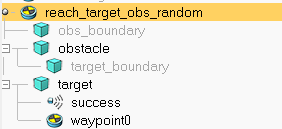
\includegraphics[scale=0.5]{assets/early-work/obs-random-scene-hierarchy.png}
    \caption{`ReachObs\_Random' Scene Hierarchy}
  \end{subfigure}
  \hfill
  \begin{subfigure}{0.45\linewidth}
    \centering
    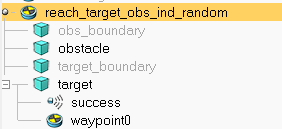
\includegraphics[scale=0.5]{assets/early-work/obs-ind-random-scene-hierarchy.png}
    \caption{`ReachObs\_IndRandom' Scene Hierarchy}
  \end{subfigure}
  \caption{Reaching Task with an Obstacle}\label{fig:reach-obs-random}
\end{figure}\todo[color=blue]{smaller?} 

\subsection{Running the Task}
There were a few interesting things of note happening on this task. 

I used the unchanged reaching policy from earlier\todo{ref}. Unsurprisingly this did not perform amazingly, however, there are some important lessons to learn form what we are seeing here. Firstly, I adopted to observe the `minimum distance' to target this time \ref{fig:ro-random-cams}, however the `final distance ' graph can be found in the appendix \todo[color=green]{link appendix}. 

\subsection{Why is `IndRandom' just worse?}\todo{not sure actually}
I did not include any figures here as there were too many\todo{should i include figures here}, however some nice ones can be found in \todo{ref the appendix}. To summarise

\begin{figure}[htpb] % htpb allows all placement
  \centering
  \begin{subfigure}{0.45\linewidth}
    \centering
    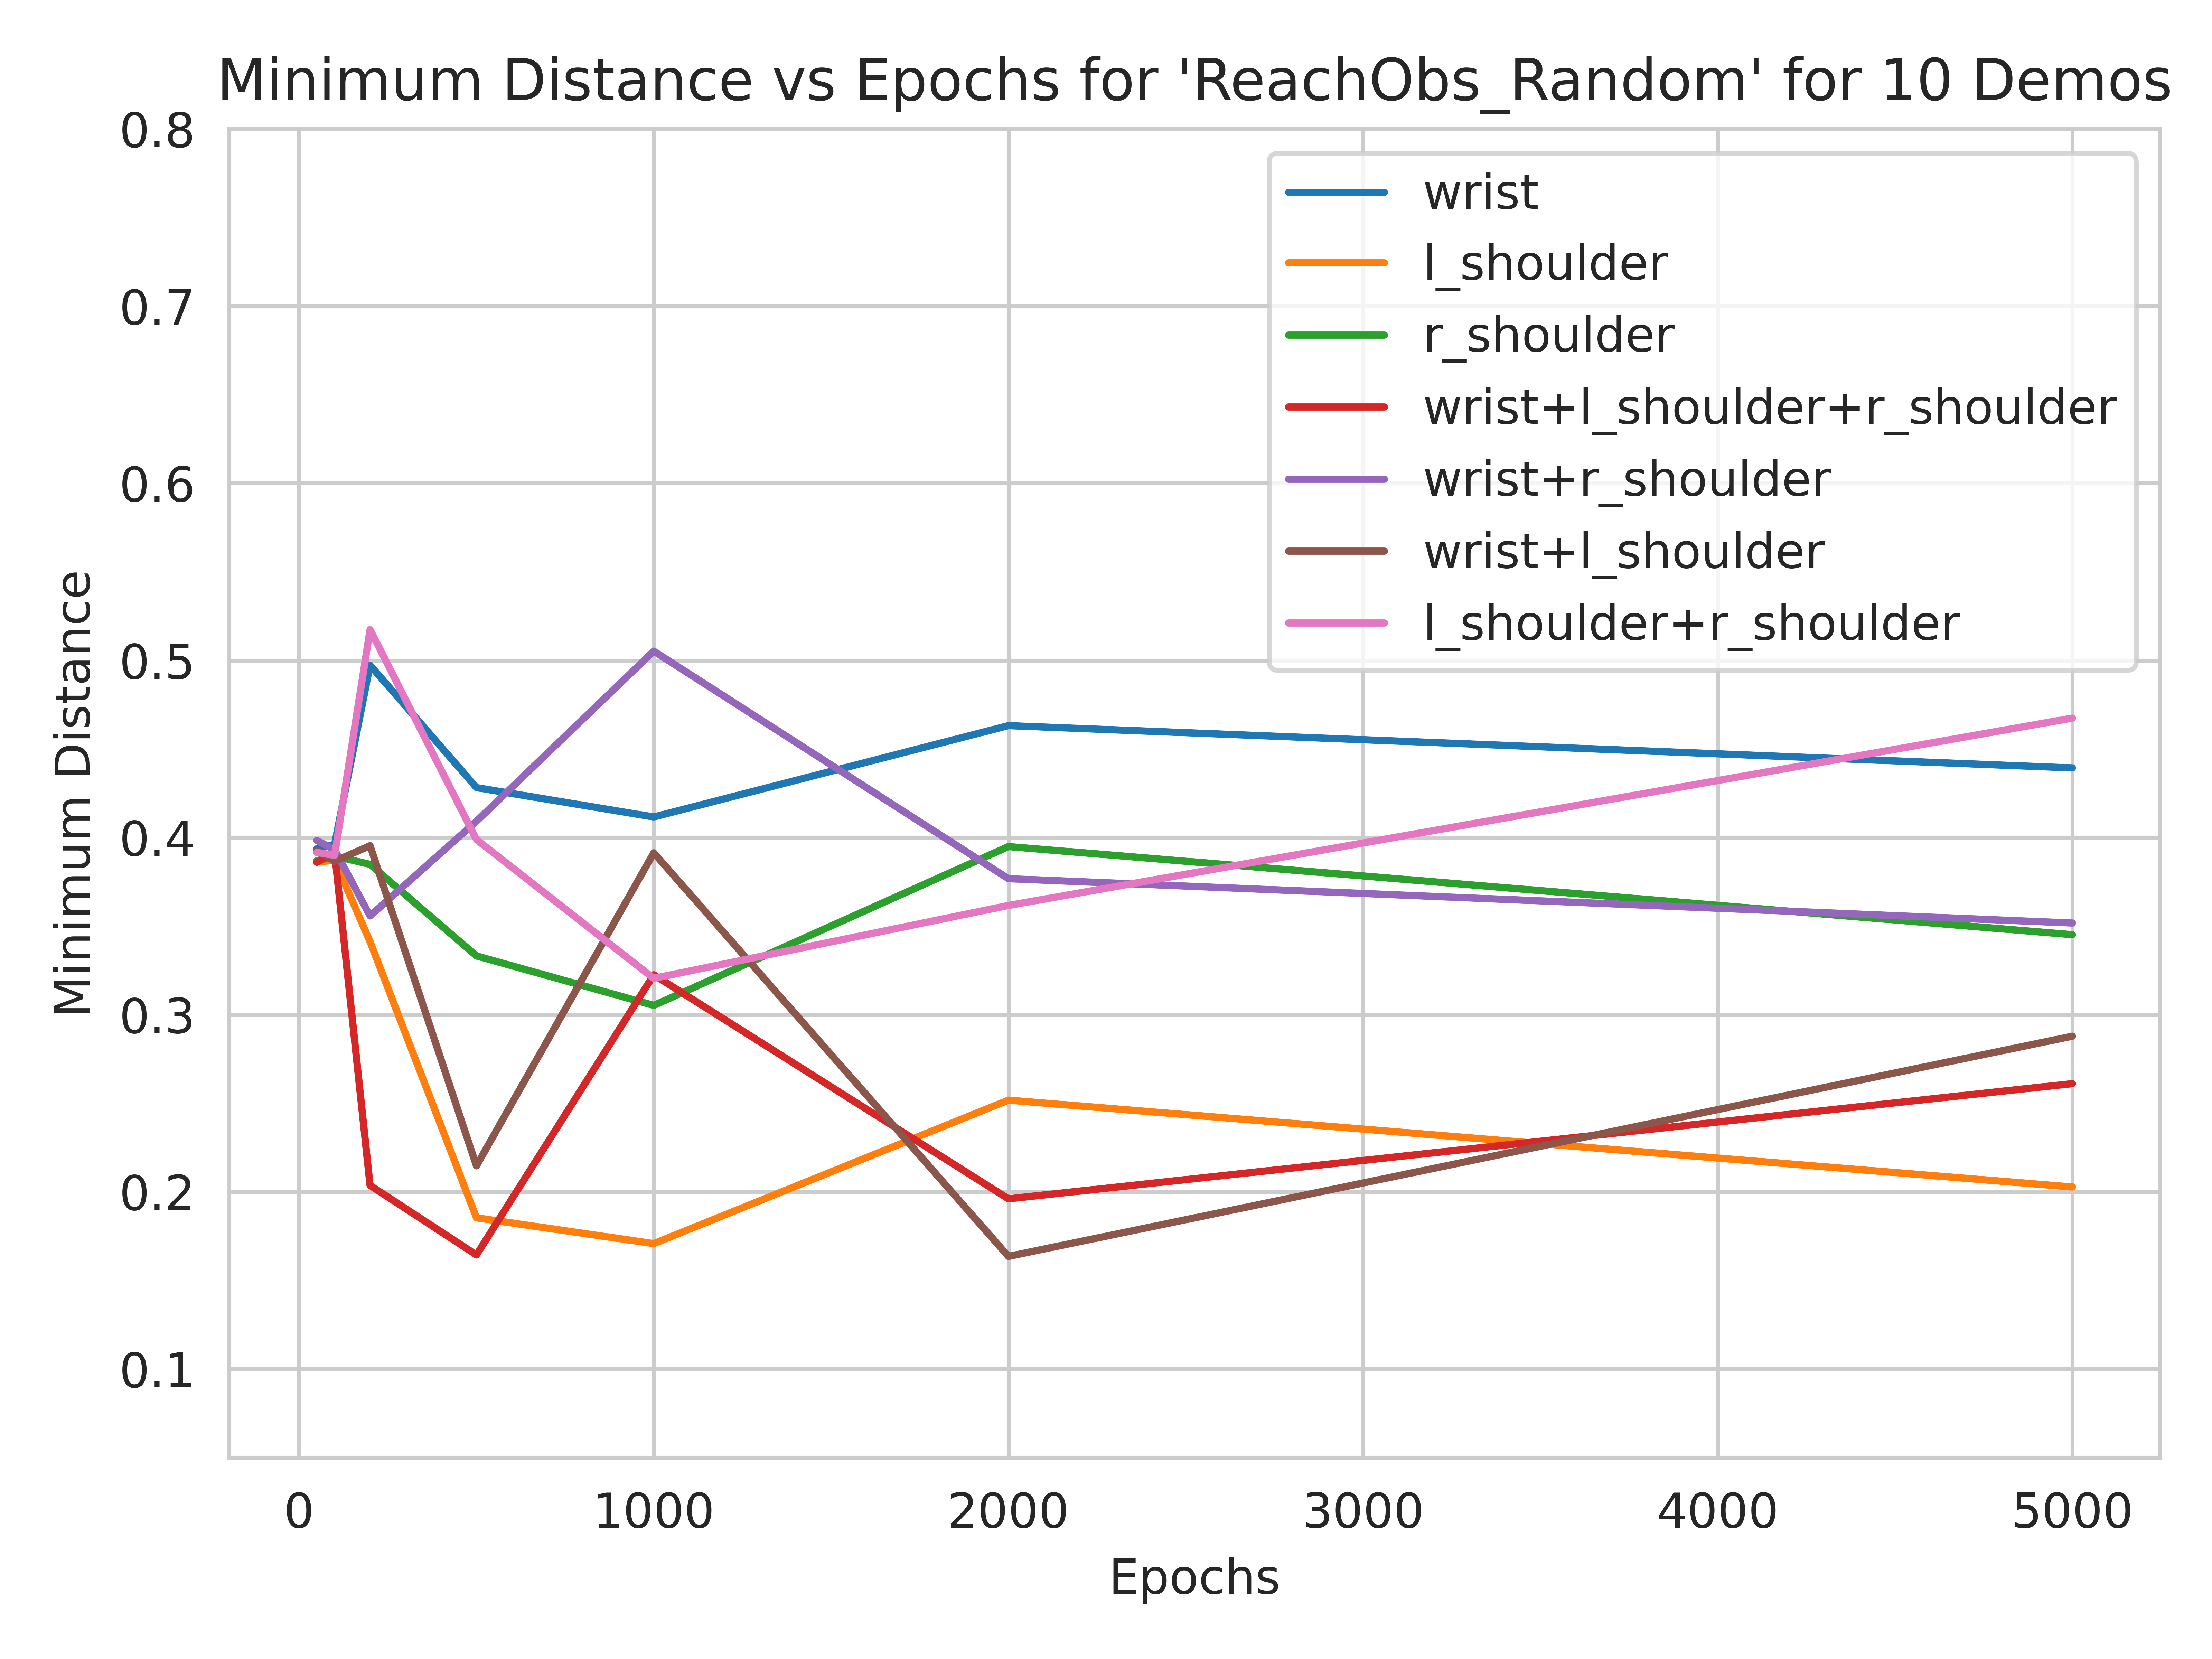
\includegraphics[width=\linewidth]{assets/cam-comb/reach-obs/ro_random-demo-mindist-10demos.png}
    \caption{Minimum Distance to Target}\label{subfig:ro-random-demo-dist20}
  \end{subfigure}
  \begin{subfigure}{0.45\linewidth}
    \centering
    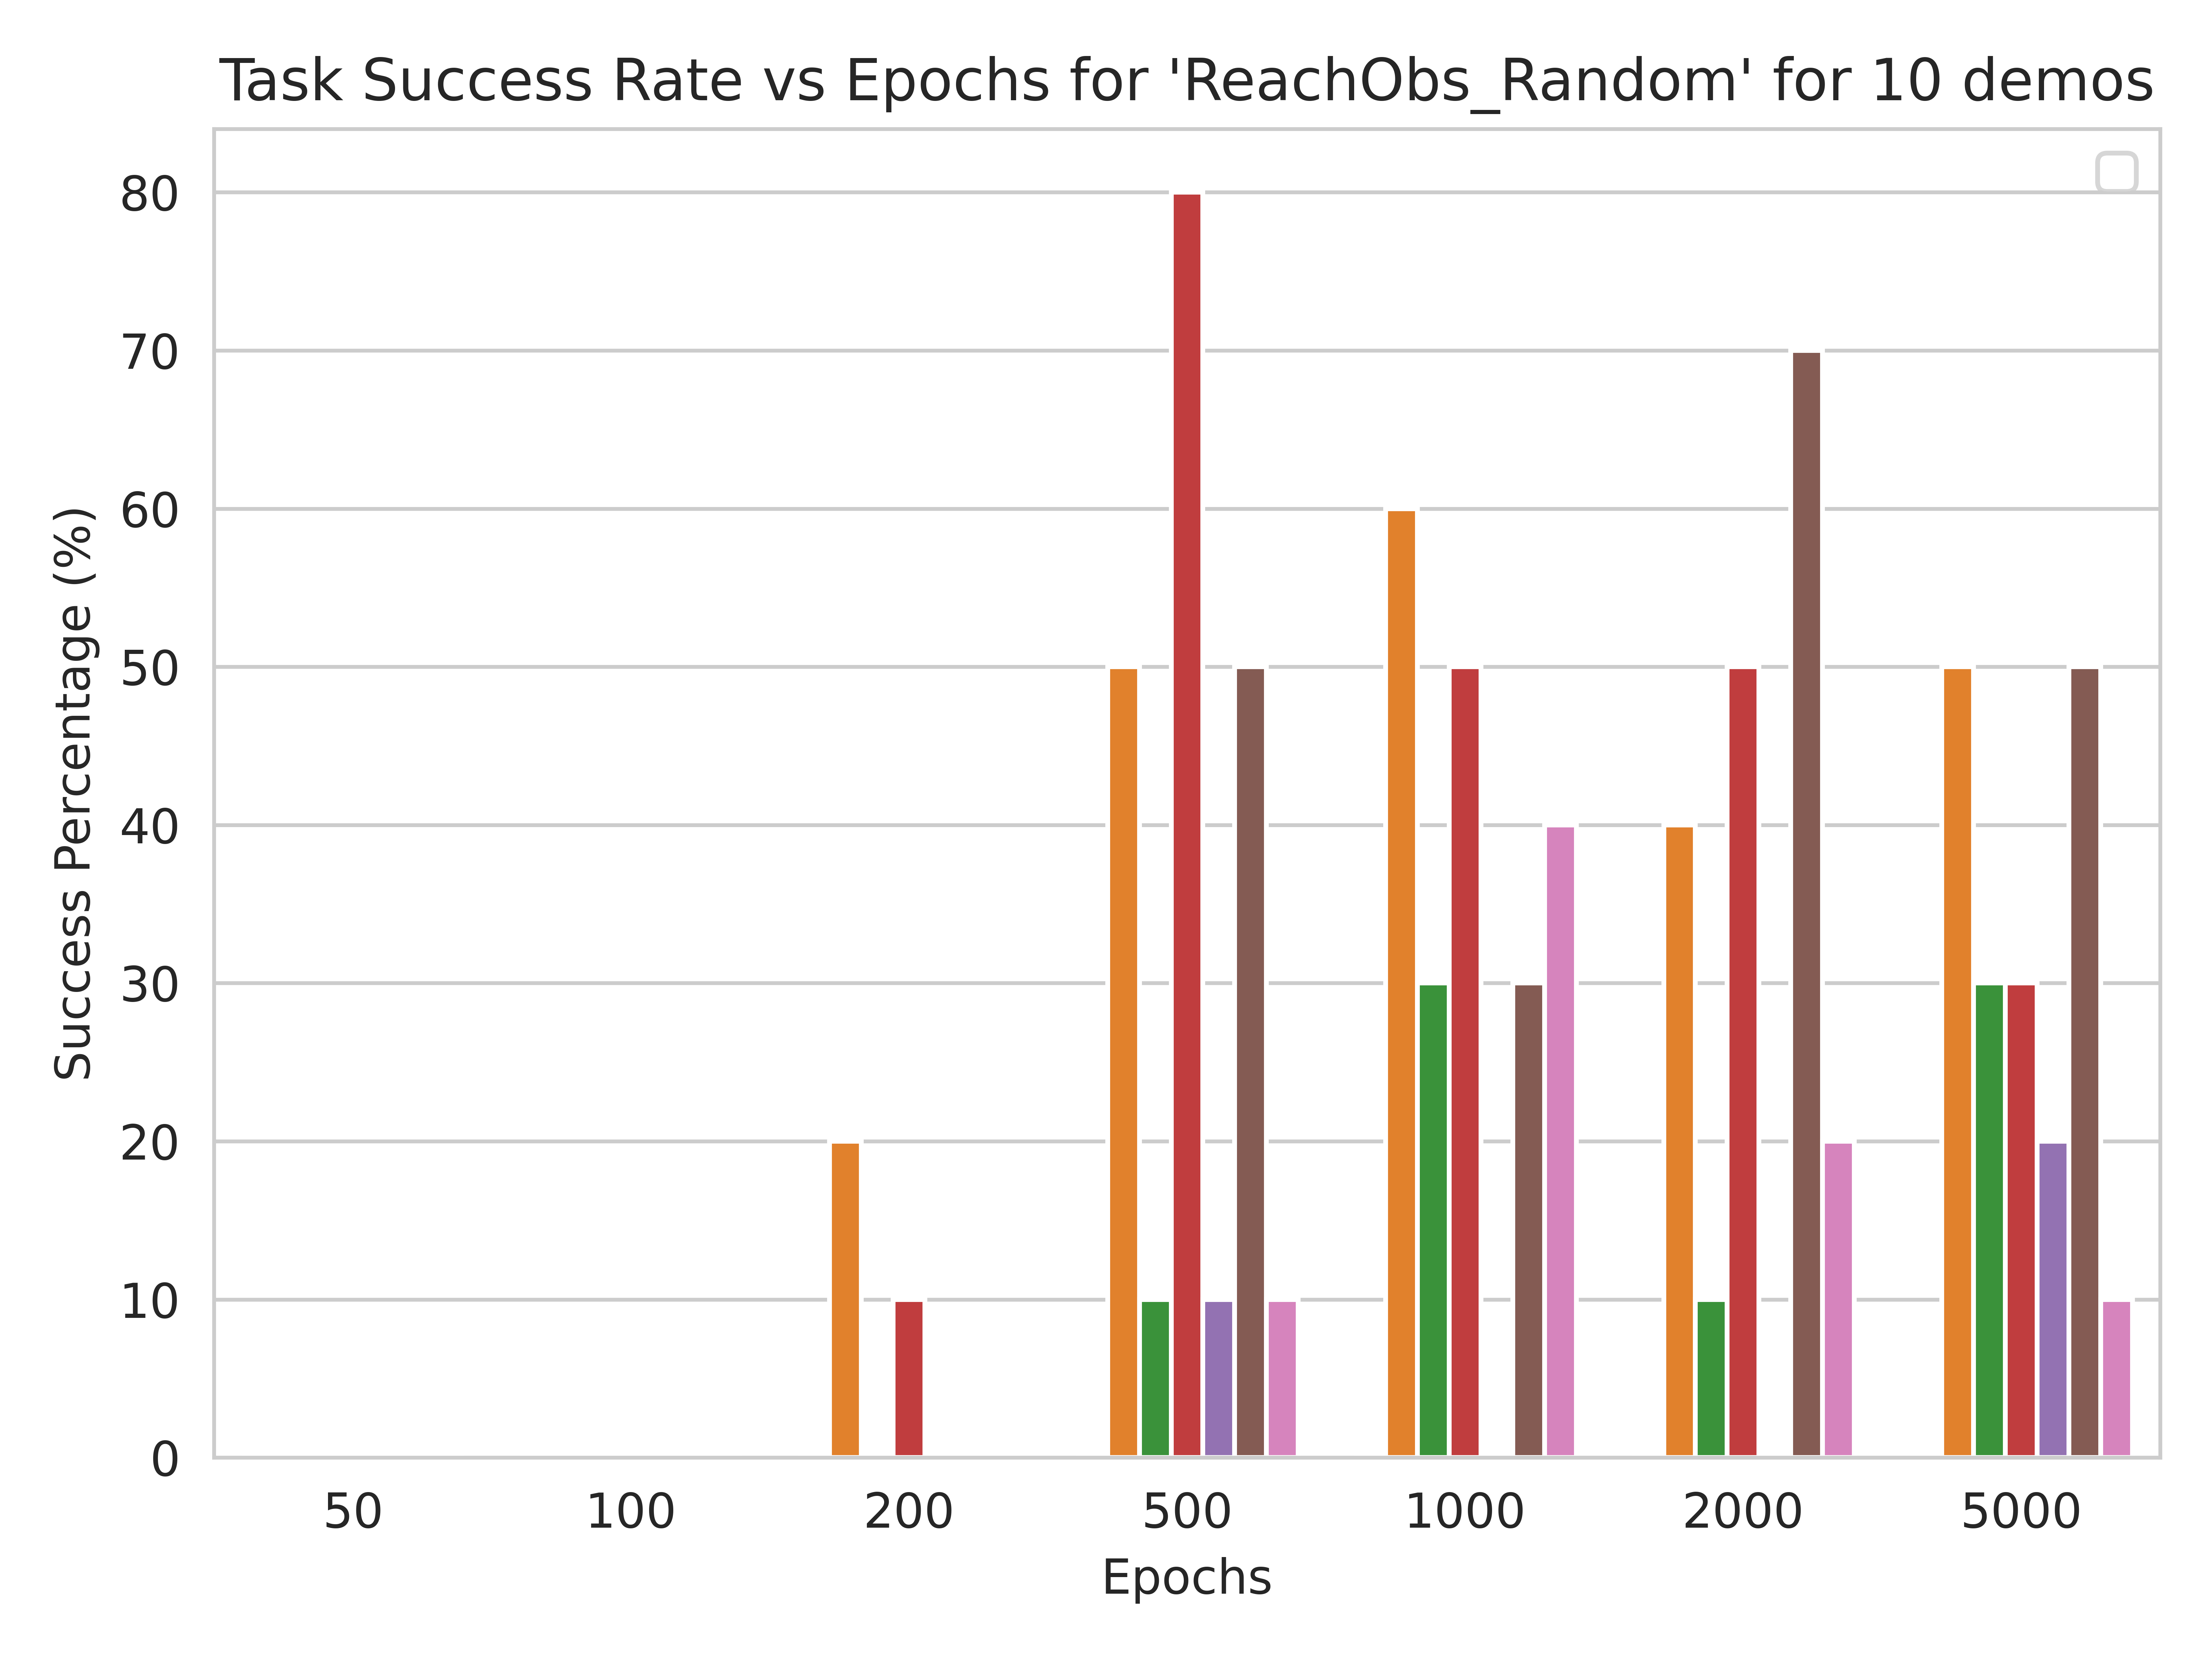
\includegraphics[width=\linewidth]{assets/cam-comb/reach-obs/ro_random-demo-success-10demos.png}
    \caption{Success Rate (\%) of Task}\label{subfig:ro-random-demo-success-20}
  \end{subfigure}
  \caption{Policy trained on 10 demos, using the \emph{demo dataset} from \ref{subsec:grasp-data-loading-changes}}\label{fig:ro-random-demo-cams}
\end{figure}

\begin{figure}[htpb] % htpb allows all placement
  \centering
  \begin{subfigure}{0.45\linewidth}
    \centering
    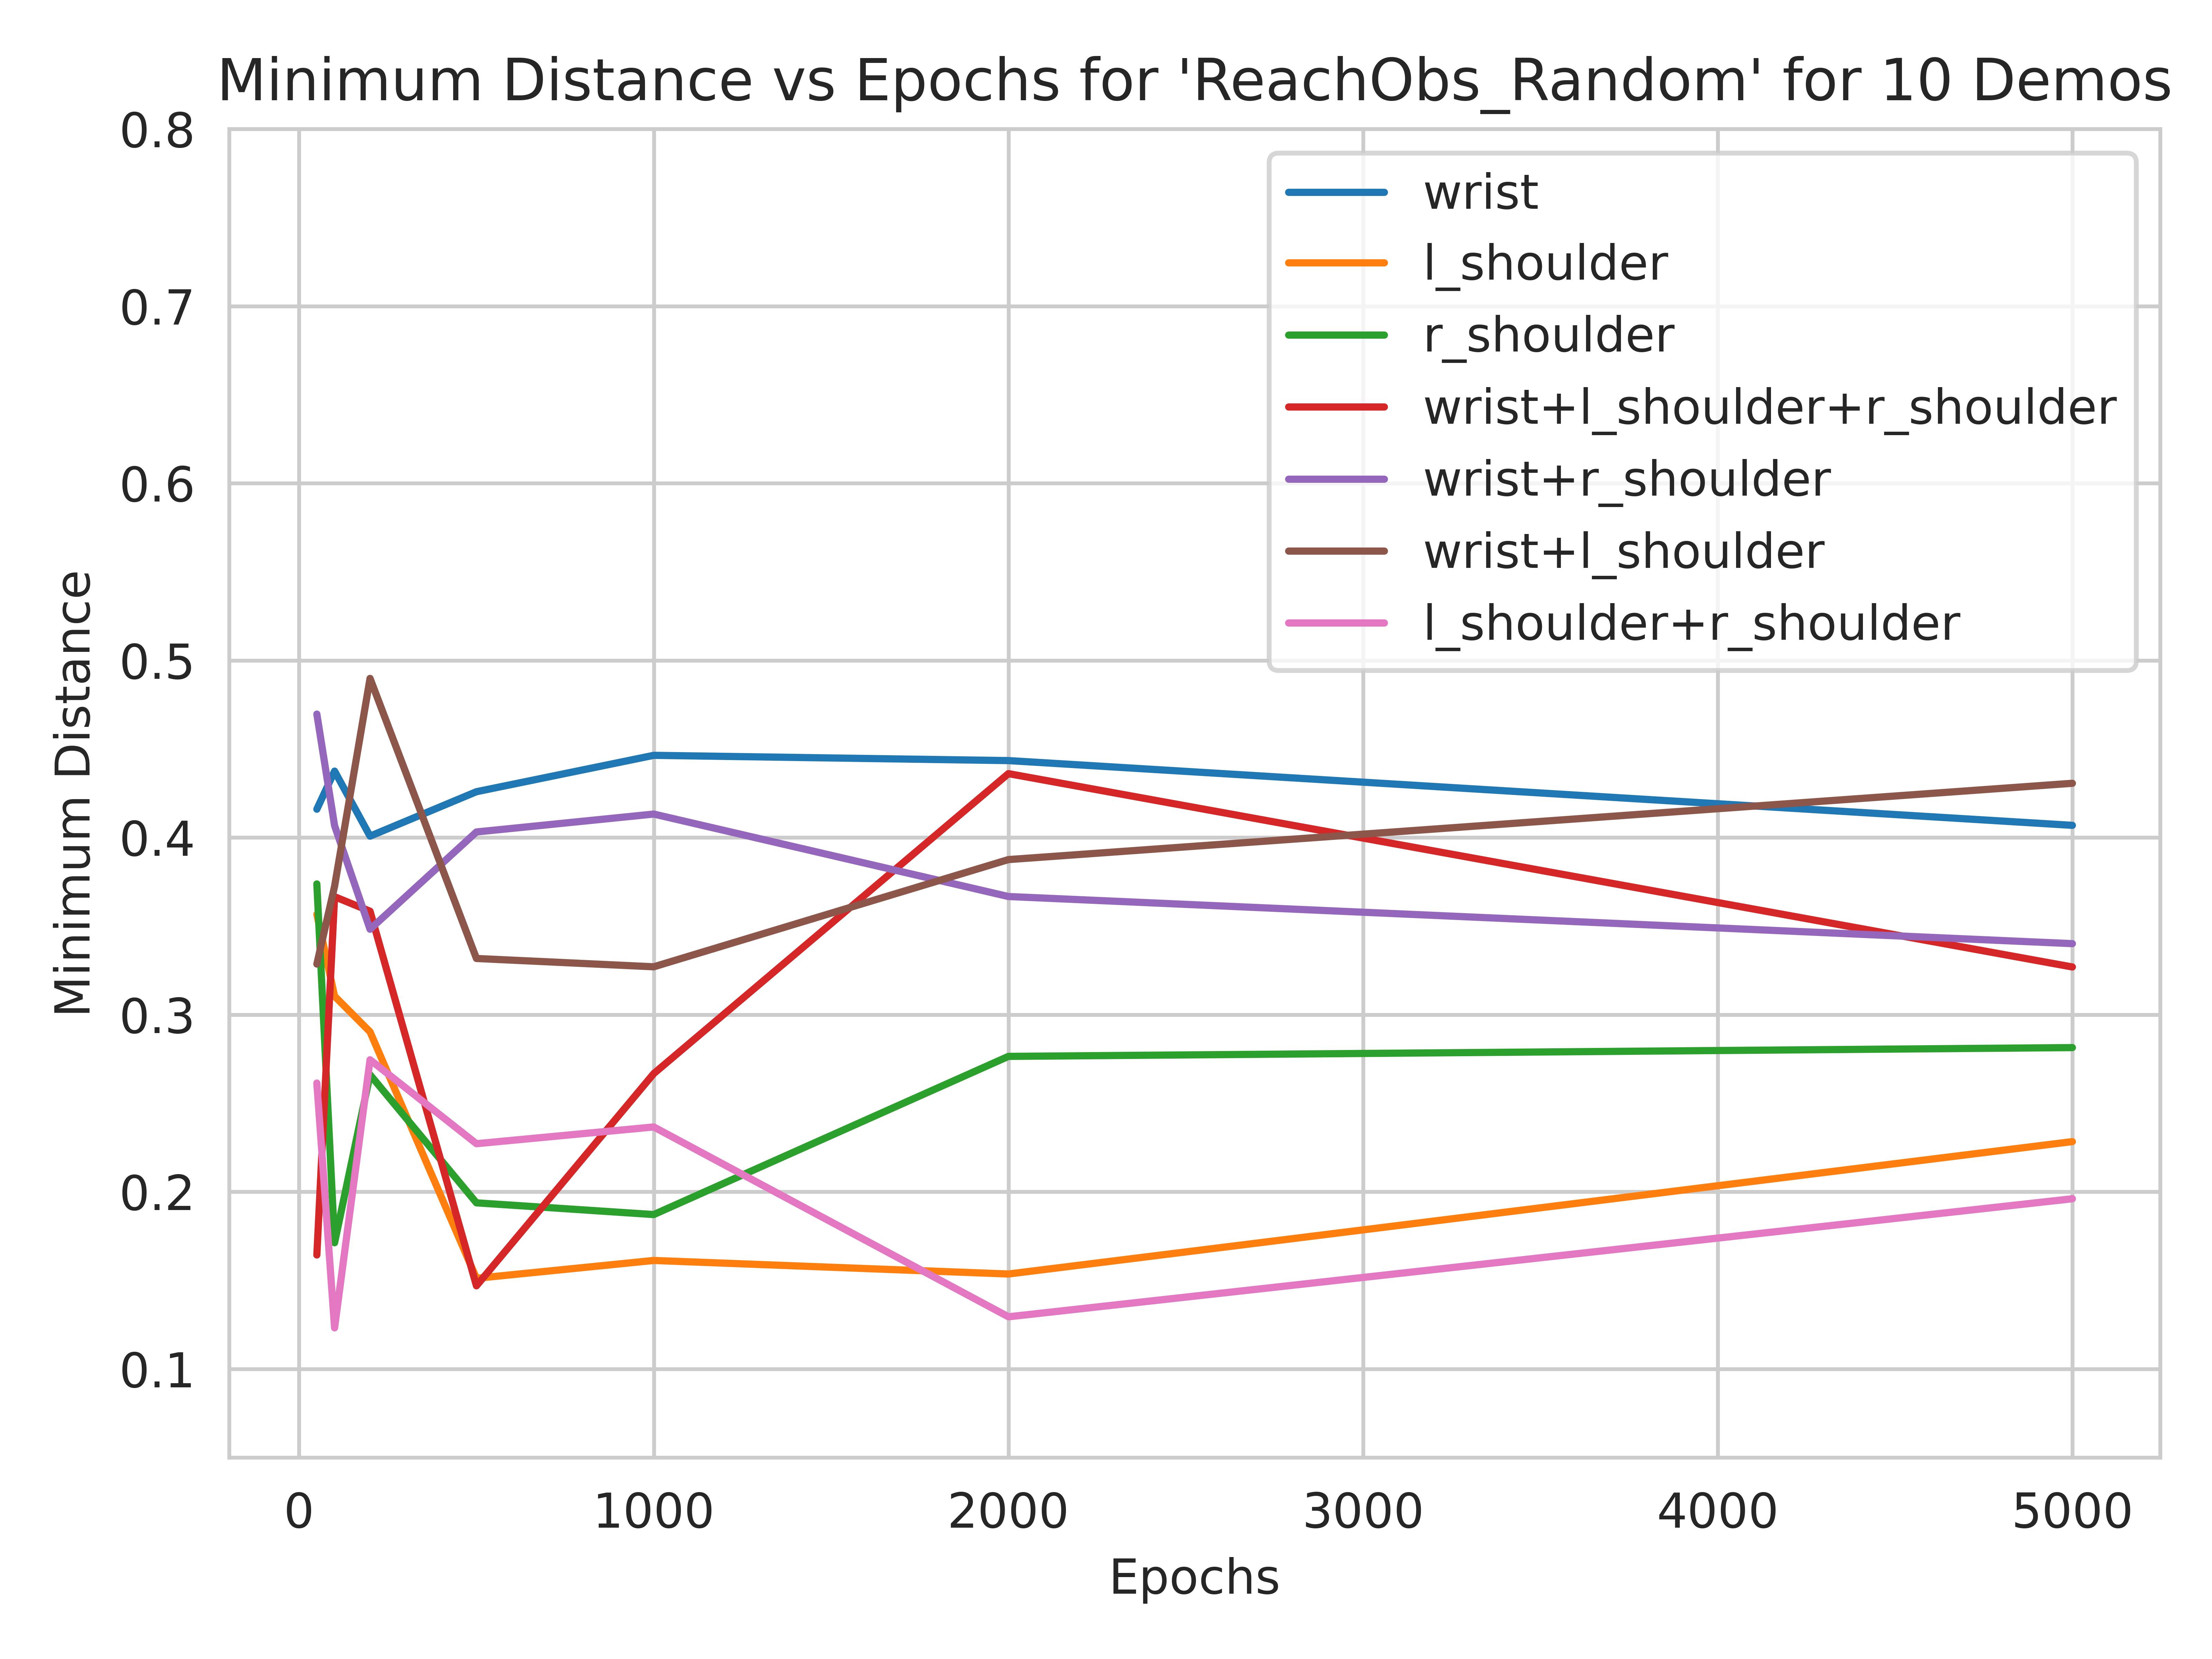
\includegraphics[width=\linewidth]{assets/cam-comb/reach-obs/ro_random-obs-mindist-10demos.png}
    \caption{Minimum Distance to Target}\label{subfig:ro-random-obs-dist20}
  \end{subfigure}
  \begin{subfigure}{0.45\linewidth}
    \centering
    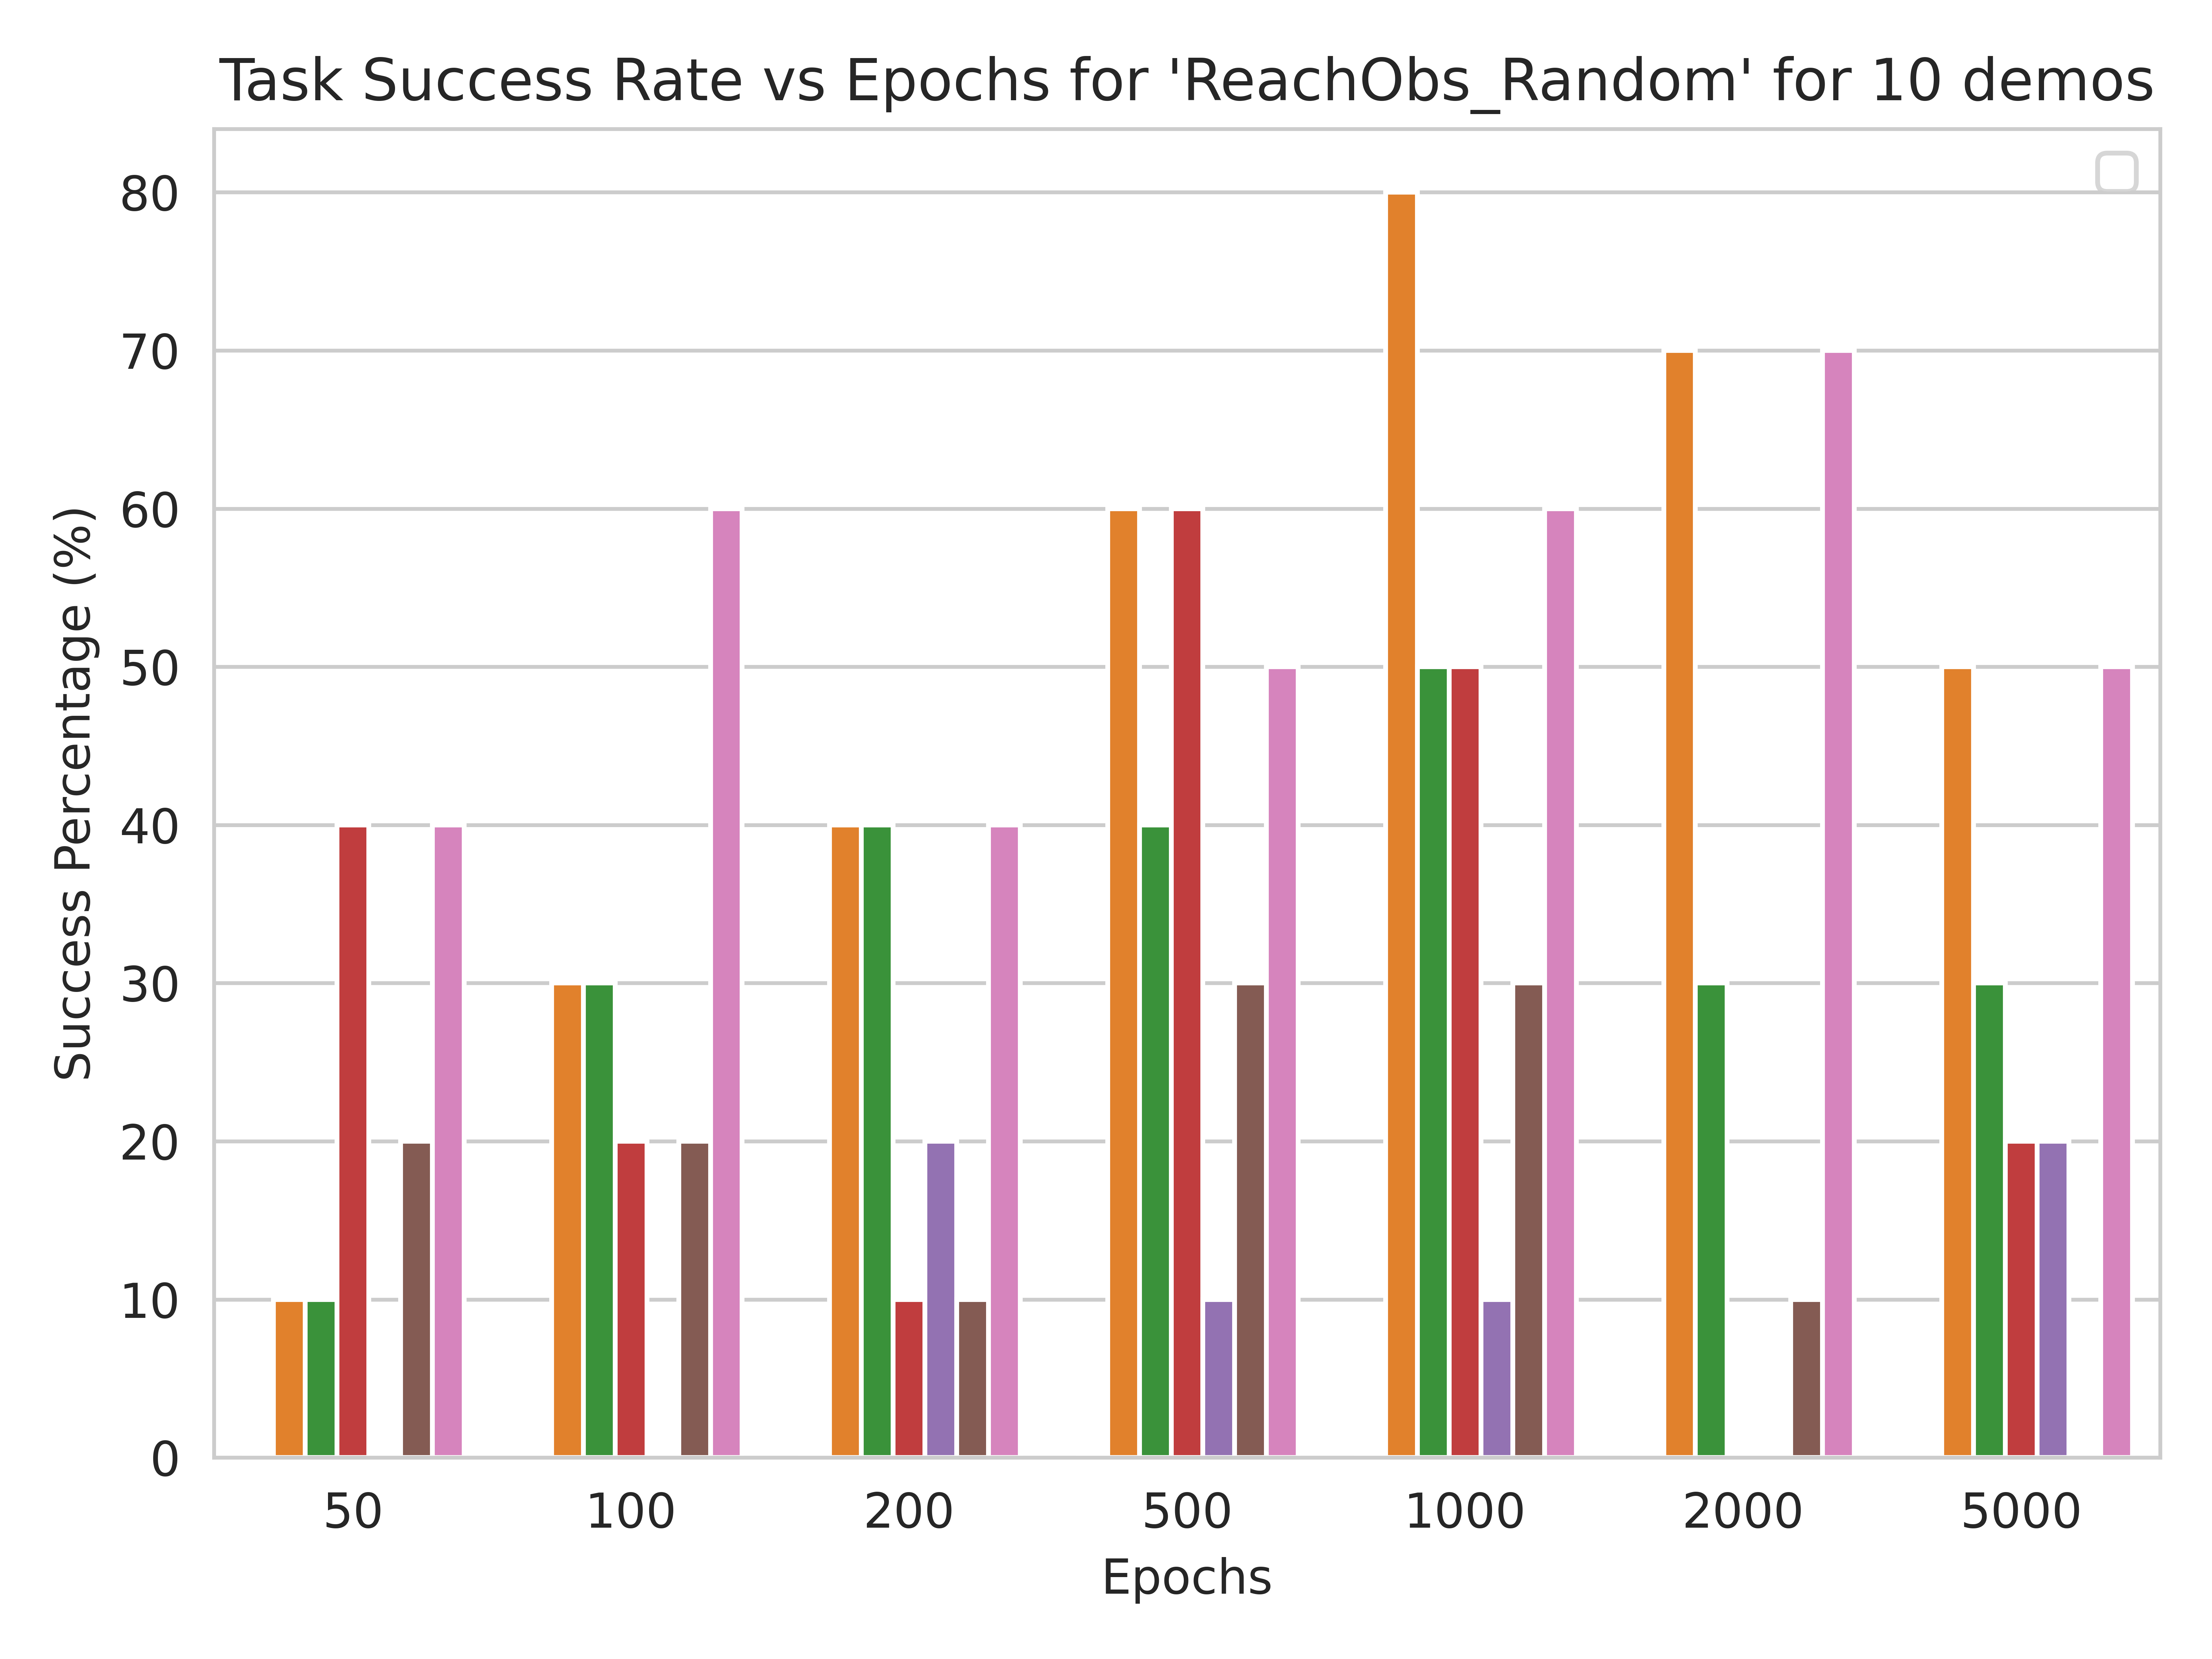
\includegraphics[width=\linewidth]{assets/cam-comb/reach-obs/ro_random-obs-success-10demos.png}
    \caption{Success Rate (\%) of Task}\label{subfig:ro-random-obs-success-20}
  \end{subfigure}
  \caption{Policy trained on 10 demos, using the \emph{obs dataset} from \ref{subsec:reach-data-loading}}\label{fig:ro-random-obs-cams}
\end{figure}



\subsubsection{Understanding the Data Management}\todo{explain the weirdness of the demo working worse}
I had initially designed the system to flatten the given demonstrations and then draw from them during the training. However, one drawback with this is that we cannot incorporate any shuffling in the data.\todo[color=purple]{}

\subsection{Improvements}



\subsubsection{Wrist Camera Alone isn't Enough}
As expected this is where the single wrist camera started showing its shortcomings. The agent would easily move around the obstacle, however, would struggle to make the last steps in touching the target. This is mostly due to the fact that the demonstrations (which are provided by RLBench) are not necessarily pointing the wrist of the robot and hence the camera mounted there to look towards the target. This means that the behavioural cloning agent learns to to the swaying motion around a large grey body, however, is not aware of the obstacle, or even understand the task is related to reaching for the obstacle and depends on its visual cues. 

\todo{add graph of going around the obstacle but not quite reaching the target (wrist)}
\todo{show this with other combinations of cameras, comment on if the l/r without wrist can learn to go around the obstacle easily? maybe not, generalisation might be hard with no wrist}

From experiments I have realised that it learns to move around the obstacle easily, using simple behavioural cloning. However, getting the last nudge to actually reach the target is where it falls apart, especially in more realistic scenarios where the target is randomised behind the obstacle. For static placement behind the wall, the agent, expectedly is quite good. \todo{maybe explain or evidence this, plateaus aroudn the same distance value and watchig t heroot act comfirms this}

\subsubsection{Other Cameras}\todo{rename}
So, we can confirm that the wrist camera alone is not sufficient \todo{ref}, and the combination of wrist and other cameras are almost always better as more coverage of the workspace guarantees less occlusions and more information the agent can work with to make decisions. It was clear that the wrist camera alone wasn't going to cut it unless it learnt to look towards the target, so that inherently some target understanding can be encoded into a task.\todo[color=red]{looking at he target??}


\todo{talk about the policy using differnt camera inputs to blend and make informed choices? maybe some plots here showing if it is better or not?}

\todo{this is important for plan2 later, as that would depend on such a mechanism, hint and even link that from here}

\subsubsection{Implementing `Looking' into the Demonstrations}\todo{haven't done this yet}\label{ew-looking-at-target}
issues this is not easy might be working on this as a part of approach 2 later
Another solution might be to experiment with the demonstration system to make sure we are pointing the wrist camera (so, the hand of our robot) towards its target as a demonstration trajectory is calculated \todo{explain that this proved tricky and might not even be worth it}

If we can't implicitly encode the `looking' information through the demonstration that means we will have to inject this information into our agent some other way. Another way to make sure agent understands to look at the target is teaching it to actively seek out its target, either following previous works such as \todo{find some prior info tracking works add ref} where object priors are incorporated into the learning or with attention mechanisms that figure out what is important in a task without prior object information \todo{maybe reference this later}.  

\subsection{Attending on a Camera in Given Combination}
One of the first ideas, that was bordering on `active vision' was to selectively accept the encoding from a single camera depending on what it was seeing. 


\todo{talk about the implementation of the }
\subsubsection{MultiCNN}
\todo{explaint the implementations, maybe connect to }
\subsubsection{SingleCNN}
I initially though to disconnect the convolutional network, thinking the information can be encoded per view and then fused together to assign better meaning to the given pose. However, with the same logic the scene is still the same scene and encoding features together means that the network will learn to \todo{find a nice way to say the network will learn its fusing in the conv layers. maybe make sure it can}